\section{Background}\label{sec:background}

\begin{itemize}
\item General introduction: Cellular and local networks, \ac{IoT}, \ac{M2M}, \ac{D2D}. Why Cooperation?
\item Specific introduction: Data multicasting, tools for simulation of network coding, Multihop for data dissemination.
\item Specific problems to that should be addressed by the thesis: (i) Ideal codes for data dissemination to a large cluster of devices in a centralized manner, (ii) software tools for network coding simulations, (iii) Decentralized cooperation for spatial redudancy to enhance connectivities in multihop networks with Kodo + ns-3.
\item Introduction on network coding, RLNC and how does it help to the previous.
\end{itemize}

The exponential tendency for data demand predicted by major network providers \cite{cisco2016forecast,kremling2015presentation} is evident. The use of cellular networks for data consumption has become a widespread topic to the general audience. The reason has been the flourishement of online applications services from the last two decades such as:  Whatsapp, Viber (voice and messaging), Facebook, Twitter, Snapchat, Instagram, Google+ (social networking), YouTube, Netflix, SoundCloud, Spotify (video or audio streaming), Google Drive, Dropbox and OneDrive (data storage). Also, these applications have been developed not only for a \ac{PC} but also mobile smartphones and/or tablets that support either the Android, iOS or Windows Mobile \ac{OS}. Hence, it is expected that the data growth will continue within this market. From all these services, streaming applications that are based in multicast scenarios where a transmitter needs to serve tens, hundreds or even thousands of receivers are becoming more frequent in mobile or \ac{LAN} networks such as \ac{WiFi}. These types of scenarios pose tight requirements in terms of data throughput and delay to ensure a satisfactoring \ac{QoE}.

For the network operator, techniques that can offload the service infrastructure to cope with the data load are needed in order to satisfy this increasing demand. Further, due to network capacity constraints, the end-user might not be connected to a \ac{BS} in a cellular fashion. Instead, the connectivity might be provided by another user within the same spectrum and nearby area through a \ac{LAN}. The deployment of mobile devices without cellular coverage but in a local network is decentralized. This type of deployment will require the communicating devices to (i) employ multihop communications to ensure connectivity, (ii) use control access mechanisms to avoid interference in the local network. From the devices perspective, energy consumption due to data transmissions has become a limiting factor in terms of battery life. The reason is that mobile devices perform much more internal tasks than older devices from ten years ago. Therefore, mobile network designers need to consider mechanisms and techniques that aim for high throughput and low energy consumption both at the station and the end user devices and that are able to provide data offloading from current network infrastructures.

\subsection{Cooperative Device-to-Device Communications in Wireless Networks}

The concept of cooperation in wireless network has been investigated before in \cite{fitzek2006cooperation,fitzek2013mobile}

\subsection{Intra-Session Network Coding for Cooperative Wireless Networks}
Introduced by Alshwede et al. \cite{ahlswede2000network}, \ac{NC} appeared as an effective technology to remove the limitations presented previously. In this work, the authors presented a new paradigm for conveying information in communication networks. Instead of following the convention of forwarding data packets from two different data flows, the packets are mixed to create new coded packets. To decode, by receiving a coded packet and knowing the original packets, it is possible to extract the missing information. This key idea let the research community know for the first time that it was possible to code on a \textit{network} basis and not only on a \textit{link} basis as conventional \ac{FEC} technologies do.

% RLNC and applications

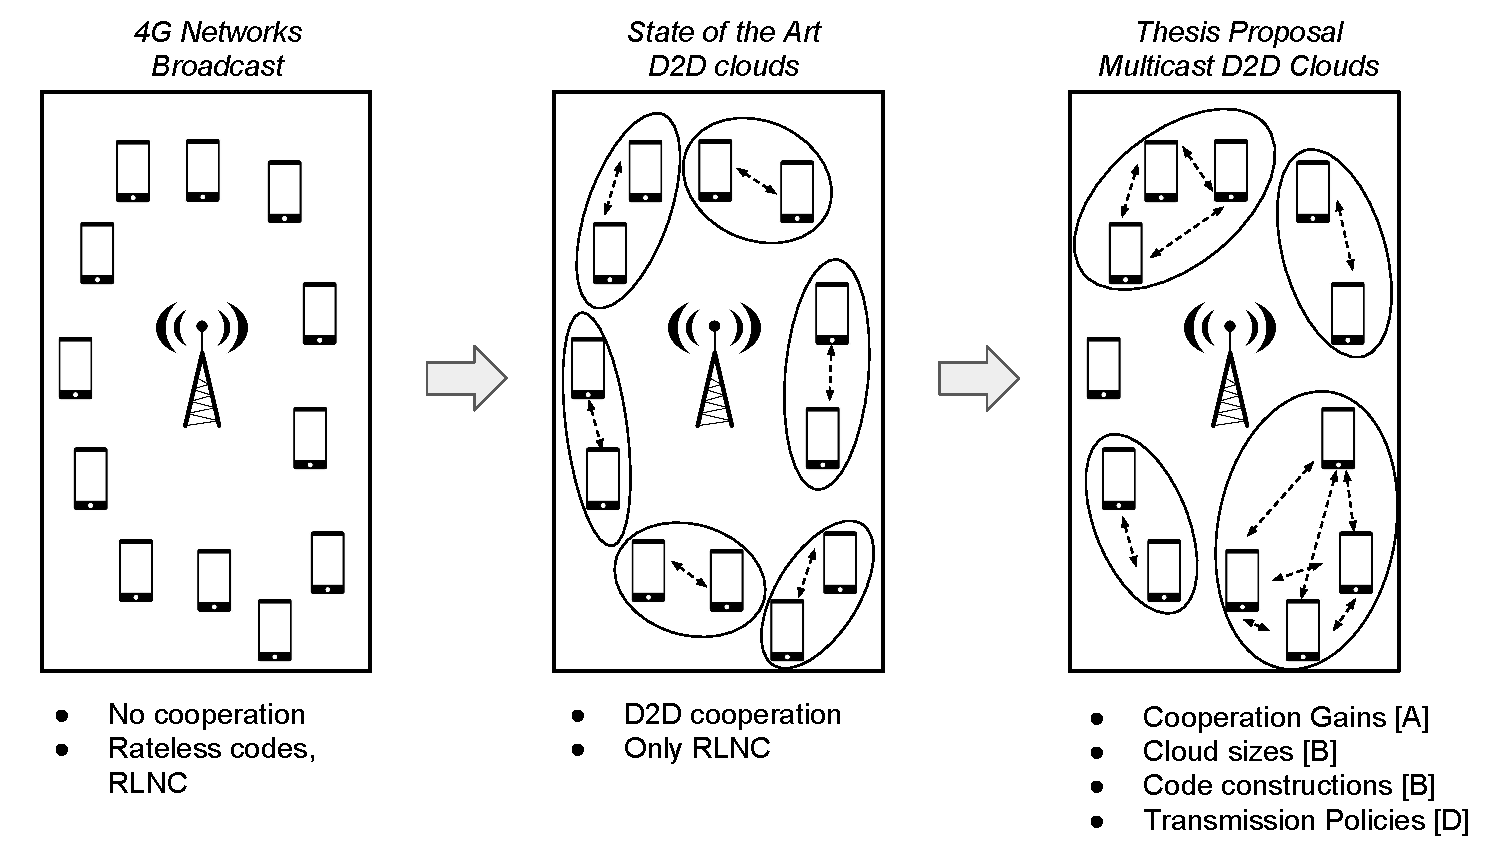
\includegraphics[width=\textwidth]{introduction/figures/thesis-diagrams.pdf}